\chapter{Elasticidad. Sólidos deformables}

\section[Propiedades elásticas. Ley de Hooke]{Propiedades elásticas. Ley de Hooke\sectionmark{Ley de Hooke}}
\sectionmark{Ley de Hooke}

El sólido está constituido por moléculas y átomos que no están quietas como el la aproximación del sólido rígido sino que en el sólido real están vibrando alrededor de sus posiciones de equilibrio.

En este tema vamos a abordar la forma en varía la estructura interna de un sólido real cuando se le somete a determinados esfuerzos; también con los fluidos, líquidos y gases.

\begin{miparrafo}
Se observa que cuando se somete un sólido real a a un esfuerzo, éste se deforma y, cuando acaba el esfuerzo, en determinadas condiciones, vuelve a su posición inicial. Esto es debido a las \emph{fuerzas elásticas}, que cuando deja de actuar la fuerza exterior deformadora, estas fuerzas de naturaleza atómica eléctrica de \emph{Van der Waals}, hacen que el cuerpo recupere su posición original.
\end{miparrafo}
	
El estudio de estas fuerzas elásticas puede tener un enfoque:

--- microscópico, que queda fuera de nuestro estudio.

--- macroscópico, comprobar como reacciona macroscópicamente el sólido real, cosa que realizó Robert Hooke en el s. XVII.


\textbf{Ley de Hooke}

\begin{miparrafodestacado}
\emph{``La deformación que se produce en un cuerpo es proporcional al esfuerzo que se le aplique.''}	
\end{miparrafodestacado}

\begin{itemize}
\item Deformación: cualquier cambio en la geometría del cuerpo.
\item Esfuerzo: cualquier causa	que contribuya a esa deformación.
\end{itemize}

\begin{multicols}{2}

La ley de Hooke es válida hasta el valor del esfuerzo $E_L$ donde acaba de ser una recta la representación \emph{esfuerzo - deformación}.

Deformación= constante x Esfuerzo; $\ y=c\cdot x\ $, donde c el la \emph{coeficiente de Hooke} o \emph{constante o coeficiente de elasticidad}.

$E_L$ es el \emph{límite de elasticidad.}
\begin{figure}[H]
	\centering
	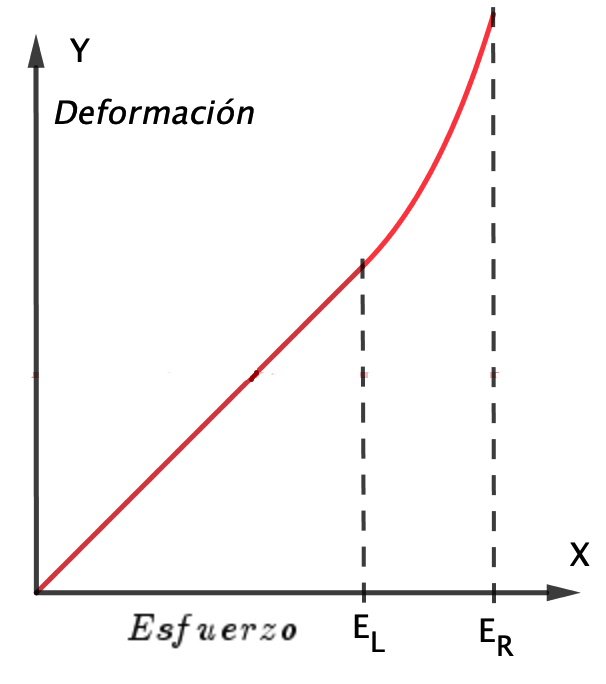
\includegraphics[width=.4\textwidth]{imagenes/imagenes09/T09IM01.png}
\end{figure}
\end{multicols}

A partir de $E_L$, para un esfuerzo mayor, el cuerpo se deforma y no recupera su estado original, quede con una \emph{deformación residual.}

Al cabo de mucho tiempo, siempre que el esfuerzo esté entre $E_L$ y $E_R$, el cuerpo logra recuperar su posición original. Este fenómeno recibe el nombre de \emph{histéresis elástica}.

A partir del valor $E_R$, \emph{carga de rotura}, el cuerpo se parte y ya no recuperará su estado original, se rompe la estructura del sólido real.

Llamamos \emph{módulo de elasticidad} a la inversa de la constante de elasticidad.

La creencia popular de `cuanto más se estira un cuerpo es más elástico' es totalmente errónea, la madera es mucho más elástica que la goma.

Líquidos y gases también presentan propiedades elásticas.

\section{Elasticidad por tracción y contracción}

\begin{multicols}{2}

Se dice que el \emph{ensayo} es por \emph{tracción} cuando la causa deformadora es una fuerza y las magnitudes deformadas son las longitudes del cuerpo en el sentido de la fuerza.

La elasticidad o el \emph{ensayo} es por \emph{contracción} cuando la causa deformadora es una fuerza y las magnitudes deformadas son las longitudes del cuerpo en el sentido contrario a dicha fuerza.
\begin{figure}[H]
	\centering
	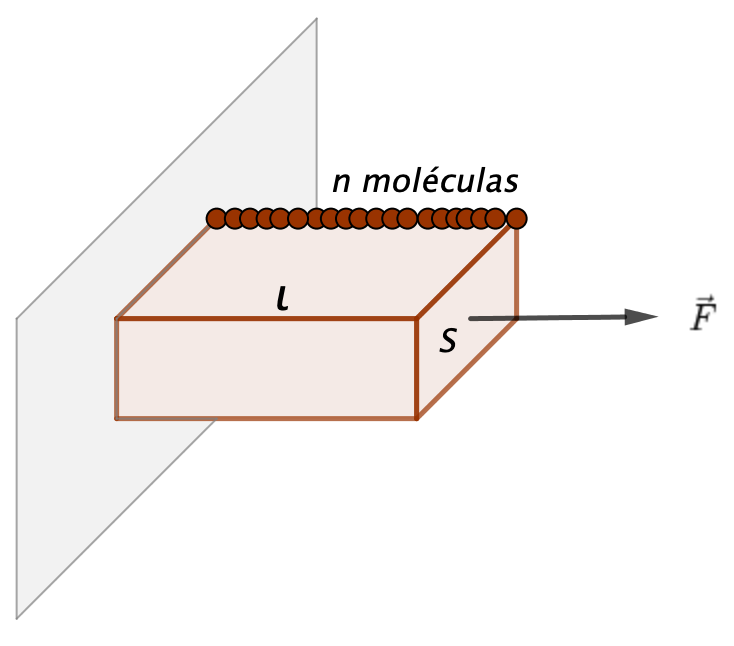
\includegraphics[width=.5\textwidth]{imagenes/imagenes09/T09IM02.png}
\end{figure}
\end{multicols}

Experimentalmente, $\ \Delta l \propto F \ $. Lo que se separan, para una fuerza $F$, las $n$ moléculas de una fila es: $\dfrac {\Delta l}{n}$ 

También se comprueba experimentalmente que la variación en longitud, $\Delta l$, es inversamente proporcional a la sección del cuerpo: $\ \Delta l \propto F \ \dfrac{l}{S}$ 

\begin{equation}
 \boldsymbol{\dfrac {\Delta l}{l} \propto \dfrac F S} \qquad \text{Ley Hooke - tracción}	
\end{equation}

La deformación, $\Delta l / l$, es proporcional al esfuerzo aplicado, $F/S$. La constante de proporcionalidad es $1/E$, siendo $E$ el llamado \textbf{\emph{módulo de Young}}.

El módulo de Young, $E$, ha de tener dimensiones de presión, en el $SI$ se expresa en $\mathrm{N/m}^2$ aunque es costumbre darlo en unidades de $\mathrm{kg} \text{ fuerza}/\mathrm{mm}^2$

Aplicamos la fuerza deformadora $F$ y, si se conserva la materia, trivialmente ha de ocurrir que al alargar el cuerpo, necesariamente, la sección final será menor que la sección inicial.

Supongamos, por facilitar el cálculo, que el cuerpo a deformar es una varilla cilíndrica de dimensiones $l$ y $r$, siendo éstas la longitud y radio iniciales.

Al aplicar el esfuerzo: $l\to l+\Delta;\quad r\to r-\Delta r$

La deformación, ahora transversal, es $\dfrac {\Delta r}{r} \propto -\dfrac {\Delta l}{l}$

Se define el \textbf{coeficiente de Piosson}, $\sigma$, (adimensional) como $\dfrac {\Delta r}{r} =\sigma \ -\dfrac {\Delta l}{l}$, por lo que la deformación transversal será:

\begin{equation} 
\boldsymbol{ -\dfrac {\Delta r}{r} =\dfrac \sigma E \ \dfrac F S } \qquad \text{Ley de Hook - tracción transversal}
\end{equation}

Resumiendo, 

--- para una \colorbox{LightYellow}{tracción}, $\Delta l>0; \ \Delta r<0$

$$\subrayado{\dfrac{\Delta l}{l}=+\dfrac 1 E \ \dfrac F S} \qquad \subrayado{+\dfrac{\Delta r}{r}=\dfrac \sigma E\ \dfrac F S}  $$

--- para una \colorbox{LightYellow}{contracción}, $\Delta l<0; \ \Delta r>0$

$$\subrayado{\dfrac{\Delta l}{l}=-\dfrac 1 E \ \dfrac F S} \qquad \subrayado{+\dfrac{\Delta r}{r}=\dfrac \sigma E\ \dfrac F S}  $$


\textcolor{gris}{$E$ Módulo de módulo de Young, $\mathrm{N\ m}^{-2}$}.

\textcolor{gris}{$\sigma$  Coeficiente de Poisson, adimensional}.

Todos los módulos de elasticidad se pueden expresa, en última instancia, como módulos de Young y coeficientes de Poisson.

\section{Compresibilidad}

Compresibilidad en sólidos, líquidos y gases.


Introducimos al sólido en el interior de un recipiente provisto de un pistón que contiene un fluido en su interior. Al comprimir el pistón, el fluido transmite la presión al sólido que queda sometido a un \emph{ensayo por compresión}.

\begin{figure}[H]
	\centering
	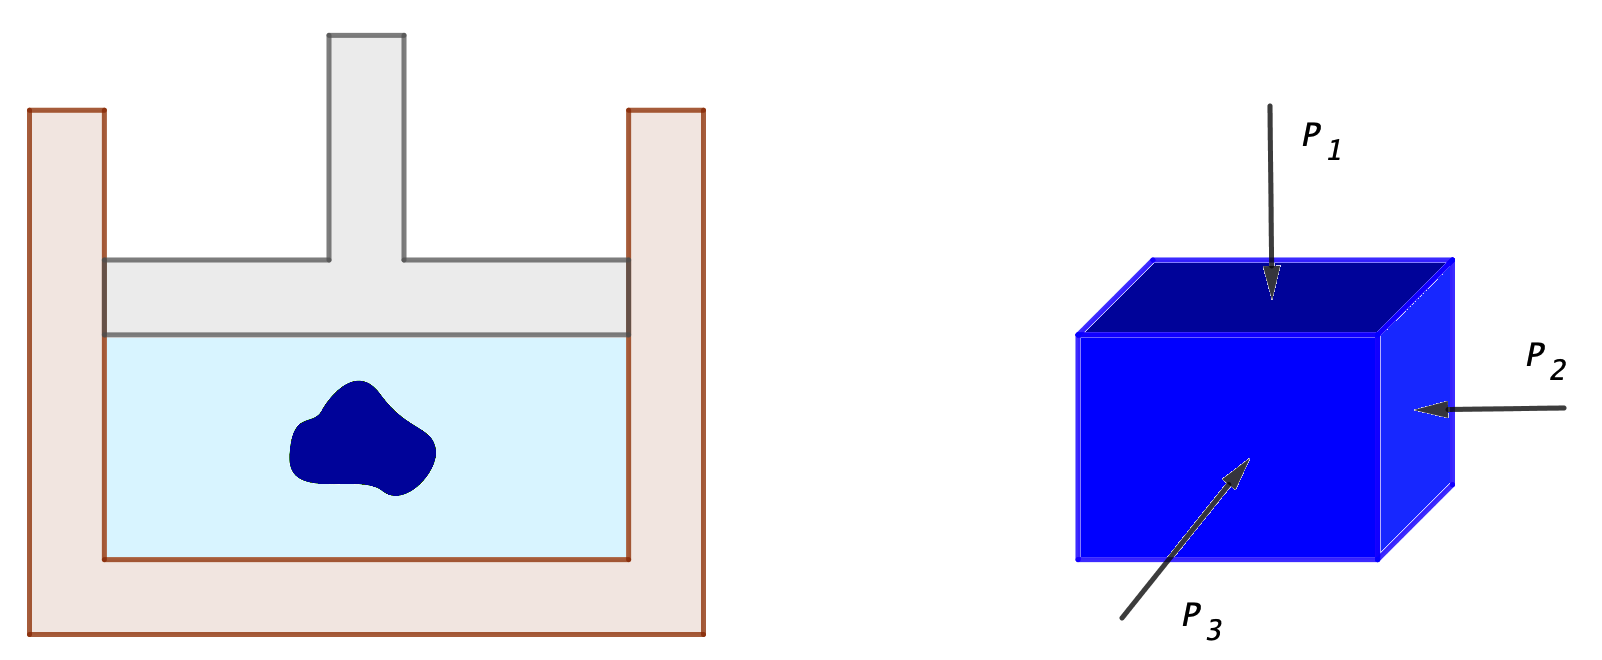
\includegraphics[width=1\textwidth]{imagenes/imagenes09/T09IM03.png}
\end{figure}

Deformación, $\Delta V/V$, esfuerzo (presión), $P$:

$-\frac {\Delta V}{V} \propto P$. En este caso, la inversa de la constante de proporcionalidad es el \textbf{módulo de elasticidad} por compresión, $Q$ y la ley de Hooke para este ensayo queda como:


$$\boldsymbol{-\dfrac {\Delta V}{V} = \dfrac 1 Q \ P} $$	

El cuerpo se comprimirá en mayor o menor medida dependiendo de su módulo de elasticidad.

Supongamos que se efectúa una fuerza $F$ en la dirección de $P_2$ sobre el cubo azul de la figura anterior. La arista en esta dirección sentirá una contracción pero las otras dos aristas perpendiculares notarán una tracción, de modo que:

$\Delta l_2=-\dfrac 1 E \dfrac{l F}{S}\;\qquad \Delta l_1=+\dfrac \sigma E \dfrac{lF}{S}; \quad \Delta l_3=+\dfrac \sigma E \dfrac{lF}{S}$
	
Luego, $\ \Delta l=\Delta l_1+\Delta l_2+\Delta l_2=\left( 2\dfrac \sigma E \dfrac F S - \dfrac 1 E \dfrac F S \right) \cdot l$

Por otra parte, $\ V=l^3 \to \Delta V = 3l^2 \Delta l; \qquad \dfrac {\Delta V}{V}=3\dfrac{\Delta l}{l}$, por lo que:

$$\subrayado{\boldsymbol{\dfrac {\Delta V}{V} = 3 (2\sigma -1)\dfrac {F}{ES}}} \qquad \text{con} \qquad \subrayado{\boldsymbol{ Q=\dfrac{E}{3(1-2\sigma)} }}$$

Expresión que proporciona la relación del coeficiente de elasticidad $Q$ con el módulo de Young $E$ y el coeficiente de Piosson $\sigma$.

Como, por definición, $Q$ no puede ser nunca negativo, ello implica que el coeficiente adimesional de Poisson ha de ser 
$\subrayado{\boldsymbol{Q<0.5}}\ $ 
\textcolor{gris}{($1-2\sigma>0)$}. 

\textbf{Compresión de un fluido}
\begin{itemize}
\item $Q$, en los líquidos, se mantiene constante para un amplio intervalo de presiones, $Q$ varía muy poco con la presión.
\item $Q$, en los gases, varía fuertemente con la presión y de distintas formas según el tipo de evolución que siga el gas: isoterma, adiabática, $\cdots$	
\end{itemize}

\subsection{Procesos Adiabáticos e isotermos}

\textbf{Procesos adiabáticos:} un proceso es termodinámicamente adiabático cuando al evolucionar un sistema desde un estado inicial hasta otro estado final no hay intercambio de energía con los alrededores.

La ecuación de estado adiabático es: $\ \boldsymbol{P \ V^{\ \gamma}=cte},\ \gamma>1$.

Diferenciando: $\ \dd P \ V^{\ \gamma}+ P \ \gamma \ V^{\ \gamma - 1} \dd V = 0$, dividiendo por $V^{\ \gamma}$

$\dd P + \gamma \ P \dfrac {\dd V}{V}=0 $, con lo que

$$\boldsymbol{-\dfrac{\Delta V}{V}=\dfrac {1}{\gamma P} \Delta P}\qquad \text{con } \  \boldsymbol{Q_A=\gamma \ P}$$

$Q_A$ es el coeficiente de elasticidad adiabático, para gases.

\textbf{Procesos Isotermos:} el cambio entre el estado inicial y final del gas se realiza a Temperatura constante. Esto se consigue haciendo la compresión muy lentamente, bajando muy poco a poco el pistón.

La ley de Boile-Mariotte dice: $\ \boldsymbol{PV=cte}$. A partir de aquí se puede demostrar que el coeficiente de elasticidad isotermo es $\boldsymbol{Q_T=P}$ (lo mismo que los procesos adiabáticos si tomamos $\gamma=1$).

\section{Elasticidad por cizayadura}

Es la deformación que sufre un cuerpo al aplicarle fuerzas tangenciales de modo que el volumen permanezca constante.

\begin{figure}[H]
	\centering
	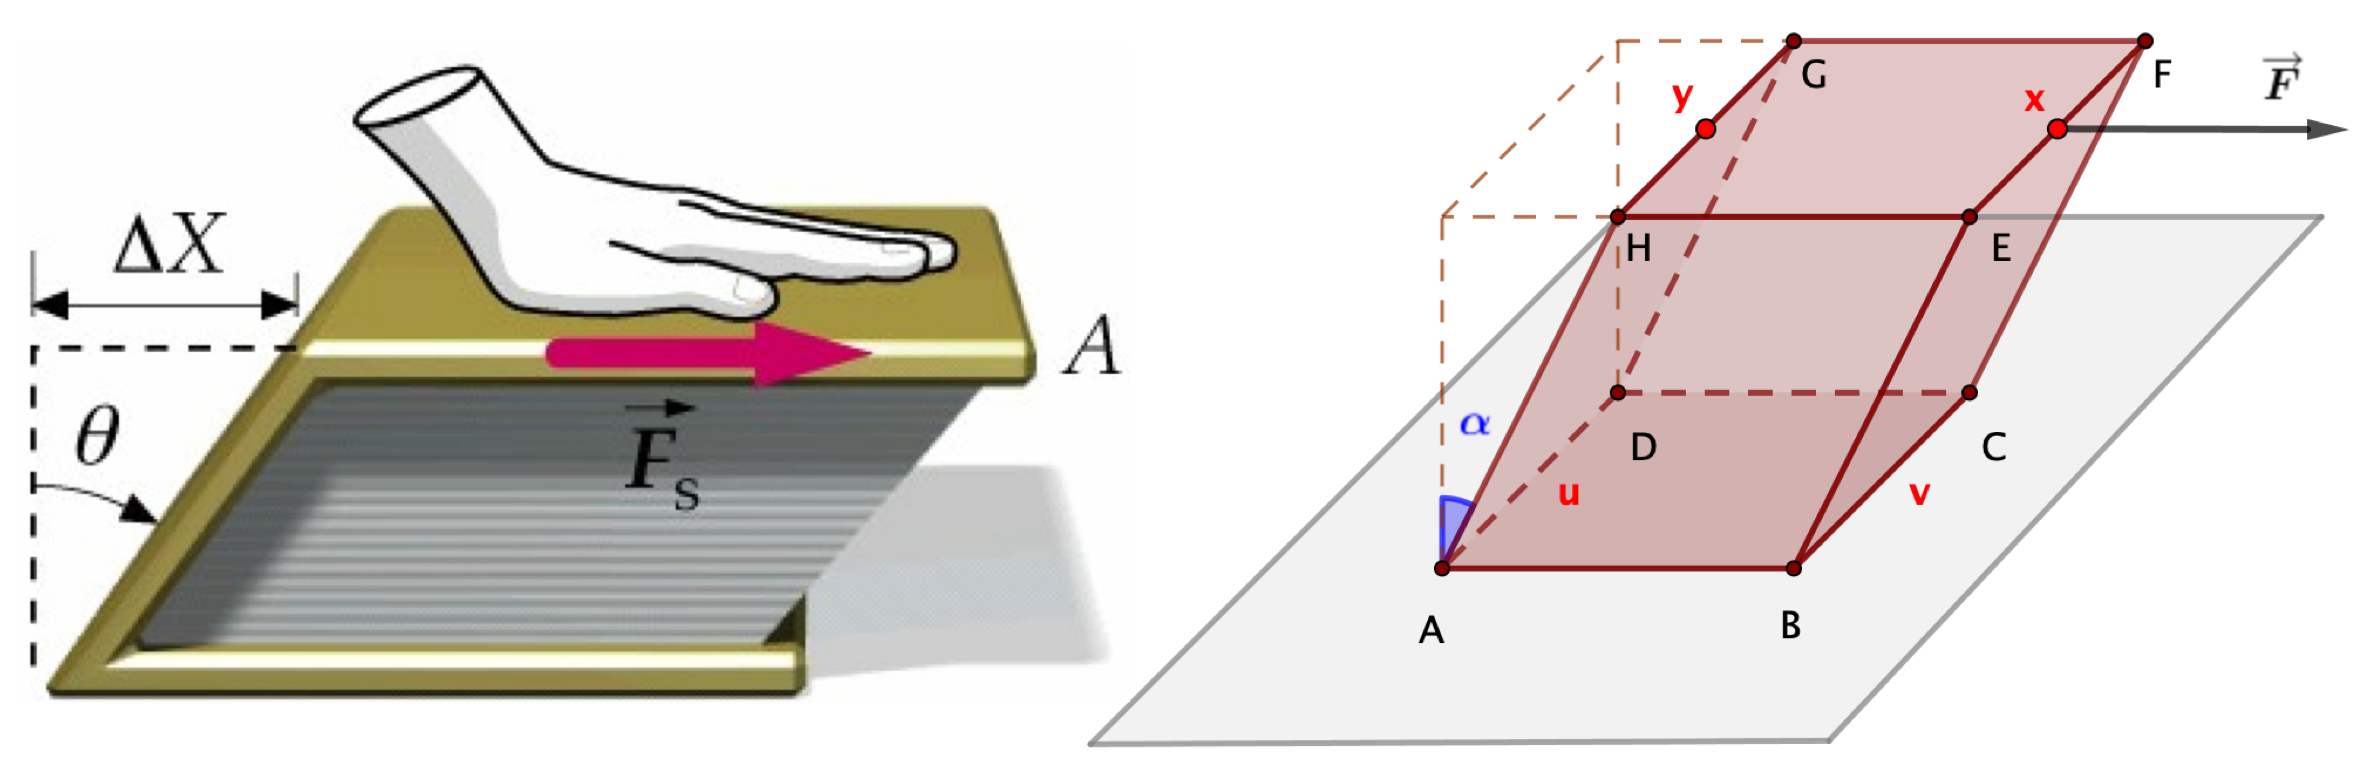
\includegraphics[width=1\textwidth]{imagenes/imagenes09/T09IM04.png}
\end{figure}

 $\alpha$ es el ángulo \emph{infinitesimal} de cizayadura, la deformación producida y es tal que $\tan \alpha \approx \alpha$  \textcolor{gris}{(infinitesimal.)}
 
 El esfuerzo aplicado lo da $F/S$, que tiene unidades de presión pero en realidad no es una presión.
 
 Es este caso:
 
 \begin{equation}
 \boldsymbol{\tan \alpha \approx \alpha = \dfrac 1 \mu \  \dfrac F S} \qquad \text{Ley Hooke - cizayadura}	
\end{equation}

$\mu$ es el modulo de elasticidad en el caso de la cizayadura.

\begin{figure}[H]
	\centering
	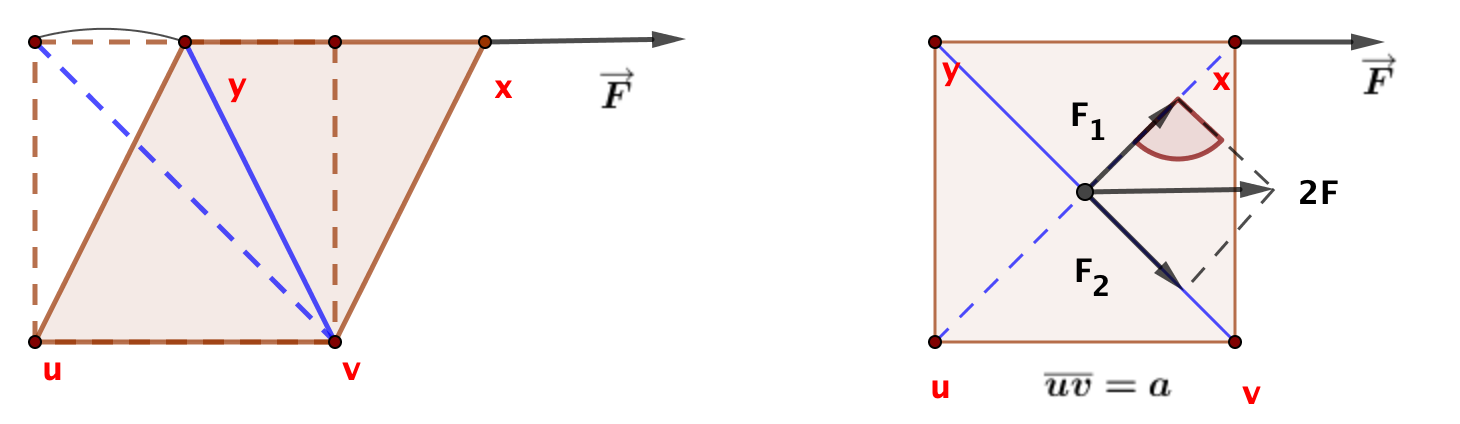
\includegraphics[width=1\textwidth]{imagenes/imagenes09/T09IM05.png}
\end{figure}

Veamos que $\mu$ depende de las caracterísrticas físicas del cuerpo, es decir, de su módulo de Young y de su coeficiente de Poisson.

Tomamos en $u$ el origen de momentos.

$a=l\sqrt 2$; $\ uv$ es el lado fijo, el cuerpo tiene la base fija en el plano. Nos fijamos en la diagonal $uv$ que pasa de medir $a$ a medir $a \pm \Delta a$

$\ast \quad$ respecto a $F_1$: la diagonal $vy$ se debe encoger, sufre una contracción:

$\Delta_1 a=-\dfrac \sigma E \ \dfrac {F_1}{S'} \ a; \quad S'=\overline{HG}\ \overline{HB}=l\ (a\ \pm \Delta a)\approx l\ a=l^2\sqrt 2=S \sqrt 2$ 

Como el ángulo de $F_1$ y $F_2$ es aproximadamente $90^o$, se tiene que $F_1\approx F_2=F\sqrt 2$

$\boldsymbol{\Delta_1 a}=-\dfrac \sigma E \ \dfrac {F_1} {S'} \ a = -\dfrac \sigma E \ \dfrac{F \sqrt 2}{S \sqrt 2} \ a =\boldsymbol{\ - \dfrac \sigma E \ \dfrac {F}{S} \ a}$

$\ast \quad$ respecto a $F_2$: la diagonal $vy$ se debe encoger, sufre una contracción (la base $uv$ está fija):

$\Delta_2 a=-\dfrac \sigma E\ \dfrac{F_2}{S''} \ a$, donde $S''=$ área $ADEF$.

Por el mismo razonamiento anterior, $S''=S \sqrt{2}$, con lo que:

$\boldsymbol{\Delta_2 a}=-\dfrac 1 E \ \dfrac {F_2} {S''} \ a = -\dfrac 1 E \ \dfrac{F \sqrt 2}{S \sqrt 2} \ a =\boldsymbol{\ - \dfrac 1 E \ \dfrac {F}{S} \ a}$

$\boldsymbol{\Delta a=}\Delta_1 a+\Delta_2 a=\boldsymbol{-\dfrac F S \left( \dfrac{\sigma+1}{E} \right) \ a}$

\begin{multicols}{2}
$\quad$

$\tan \alpha = \dfrac b l; \qquad a=l\ \sqrt 2$

$|\Delta a|\approx b \ \cos 45^o=b\ \dfrac{\sqrt 2}2=\dfrac b {\sqrt 2}$

$\alpha \approx \tan \alpha = \dfrac{|\Delta a|\ \sqrt 2}{l}=\dfrac{2\ |\Delta a|}{a}$
\begin{figure}[H]
	\centering
	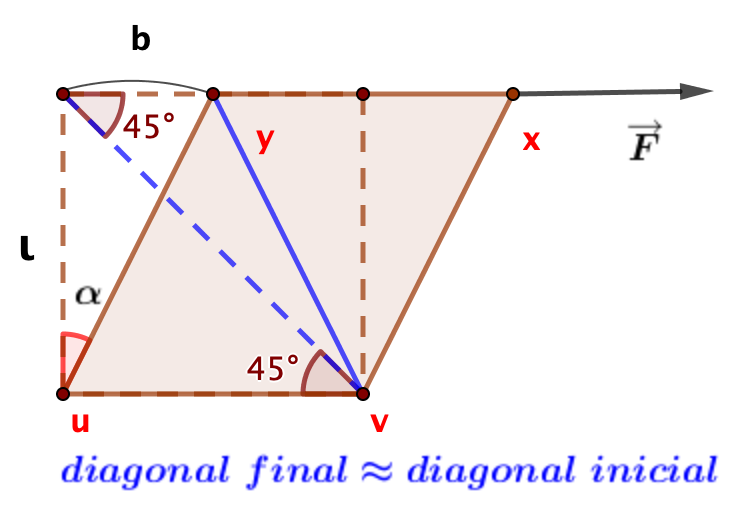
\includegraphics[width=.5\textwidth]{imagenes/imagenes09/T09IM06.png}
\end{figure}	
\end{multicols}

$\boldsymbol{ \alpha }\approx \tan \alpha = \dfrac{2\ |\Delta a|}{a}  \boldsymbol{=2 \dfrac F S \left( \dfrac {\sigma +1}{E} \right) }$

Comparando con la expresión que hemos llamado ley de Hooke para cizayadura, encontramos el módulo de cizayadura, $\mu$, en función de $\sigma$ y $E$:

$$\boldsymbol{ \tan \alpha = \dfrac 1 \mu \ \dfrac F S }, \quad \text{ con } \qquad \boldsymbol{ \mu=\dfrac{E}{2(\sigma + 1} }$$


\section{Elasticidad por torsión}

\begin{multicols}{2}
Supongamos un cuerpo cilíndrico de altura $l$ y radio $r$ sujeto por la base al cual se le retuerce. En estas condiciones decimos que le hemos sometido a un \emph{esfuerzo por torsión}.

El esfuerzo lo da el momento de la fuerza tangencial aplicada, $M=f\cdot r$.

La deformación es medida por el ángulo $\beta$, \emph{ángulo de torsión}.



\begin{figure}[H]
	\centering
	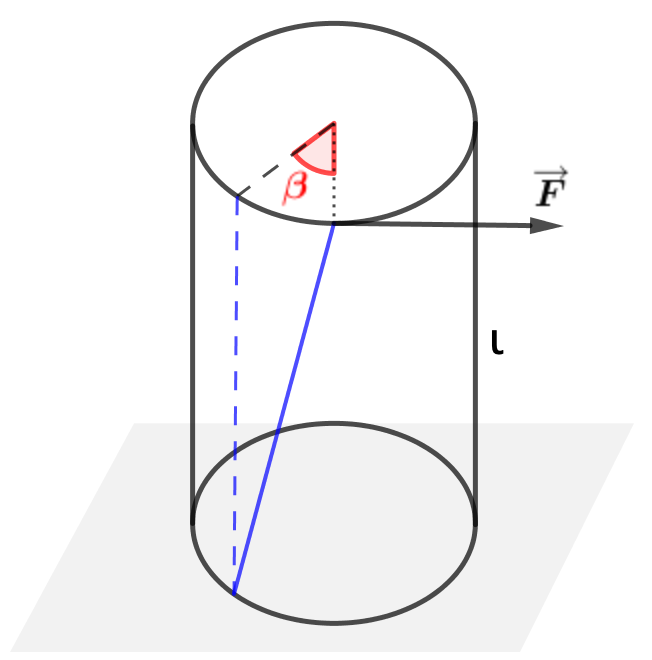
\includegraphics[width=.5\textwidth]{imagenes/imagenes09/T09IM07.png}
\end{figure}		
\end{multicols}

$$ \beta = \dfrac 1 R \ M$$

$R$ \textbf{no} es el \emph{módulo de torsión} y depende no solo de las características elásticas del cuerpo sino también de las geométricas. Una misma sustancia con la que se construyen dos hilos distintos, tienen distinta R; por eso no se llama módulo de torsión.

\begin{figure}[H]
	\centering
	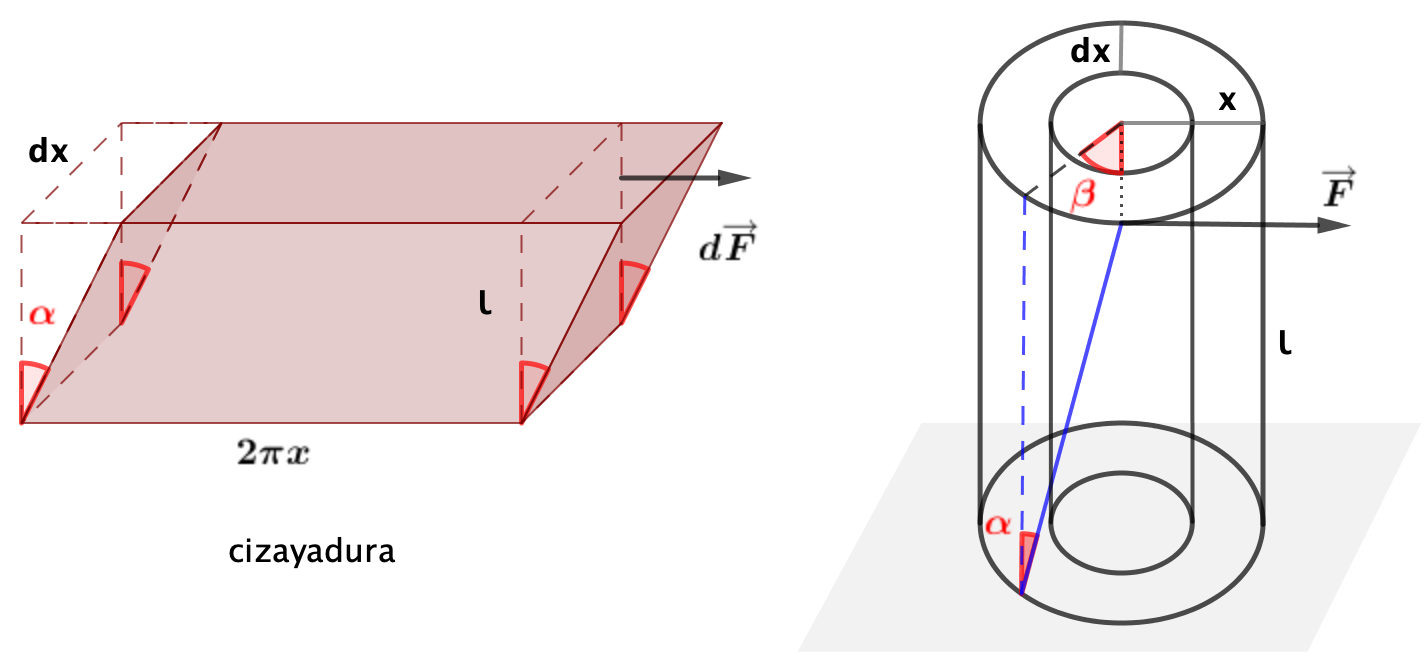
\includegraphics[width=1\textwidth]{imagenes/imagenes09/T09IM08.png}
\end{figure}	

En el plano de la circunferencia hay cizayadura:

 $\alpha=\dfrac 1 \mu \ \dfrac {\dd F}{2\pi x \dd x} \ \to \quad  \dd F=2 \pi \ \mu \ \alpha \ x \ \dd x$
 
 
De acuerdo con la ley de Hooke, $\ \dd \beta \dfrac 1 R \dd M$

$\dd M = x \ \dd F = 2 \pi \ \mu \ \alpha \ x^2 \ \dd x$

Trigonometría: $\ x\beta = l \alpha \ \to \ \alpha=x\ \dfrac \beta l$

$\dd M = 2\pi \ \mu \ \dfrac \beta l \ x^3 \ \dd x$

Integrando para obtener el momento de la fuerza aplicada al cilindro finito:

$M=\displaystyle  2\pi \ \mu \ \dfrac \beta l \ \int_{r_1}^{r_2} x^3 \ \dd x$, por lo que:

$$\boldsymbol{M= \dfrac 1 2 \pi \ \mu \ \dfrac \beta l \ (\ r_2^4-r_1^4\ )}; \qquad \beta=\dfrac 1 R\ M; \quad \boldsymbol{R=\dfrac{\mu \beta}{2l}(r_2^4-r_1^4)}$$

\textcolor{gris}{$\mu=\dfrac{E}{2(1+\sigma)}$}

\newpage %*****************************************
\section{Problemas}

\begin{prob}.

El límite elástico del cable de un ascensor es de $2.8 \times 10^{-2}\ \mathrm{kg} \ \mathrm{mm}^{-2}$. Calcúlese la máxima aceleración hacia arriba que puede imprimirse a un ascensor de $1000\ \mathrm{kg}$ sujeto por un cable de $90\ \mathrm{mm}^2$ de sección, suponiendo que el esfuerzo no debe exceder a la cuarta parte del límite elástico.	
\end{prob}

$F_{MAX}=F\ F/S = 90\cdot 2.8\ 10^{-2} \cdot 9.8 \ (*);\quad F=F_{MAX}/4=m\ a$

\textcolor{gris}{Multiplicamos por $9.8 \mathrm{ms}^{-2}$ para pasar de $\mathrm{kg}$-$\mathrm{fuerza}$ a $\mathrm{N}$.}

$a=\dfrac{F_{MAX}}{4m}=\cdots =61.74\ \mathrm{m\ s}^{-2}$

\begin{prob}.

Calcula el incremento de longitud que experimenta una barra suspendida verticalmente, bajo su propio peso.	
\end{prob}

\begin{multicols}{2}
Stookes: $\ \ \displaystyle \dv{\xi}{x}=\dfrac 1 e \dfrac {F(x)}{S}$

$F(x)=m(x)g=\rho S (L-x) g$

$\displaystyle \int_0^\xi \dd \xi = \dfrac 1 E g L \int_0^L (L-x) \dd x=\dfrac 1 E \ \rho \ g \ \eval{\dfrac{2Lx-x^2}{2}}_0^L$

$\xi = \dfrac 1 E \ \rho g \ \dfrac {L^2} 2$
\begin{figure}[H]
	\centering
	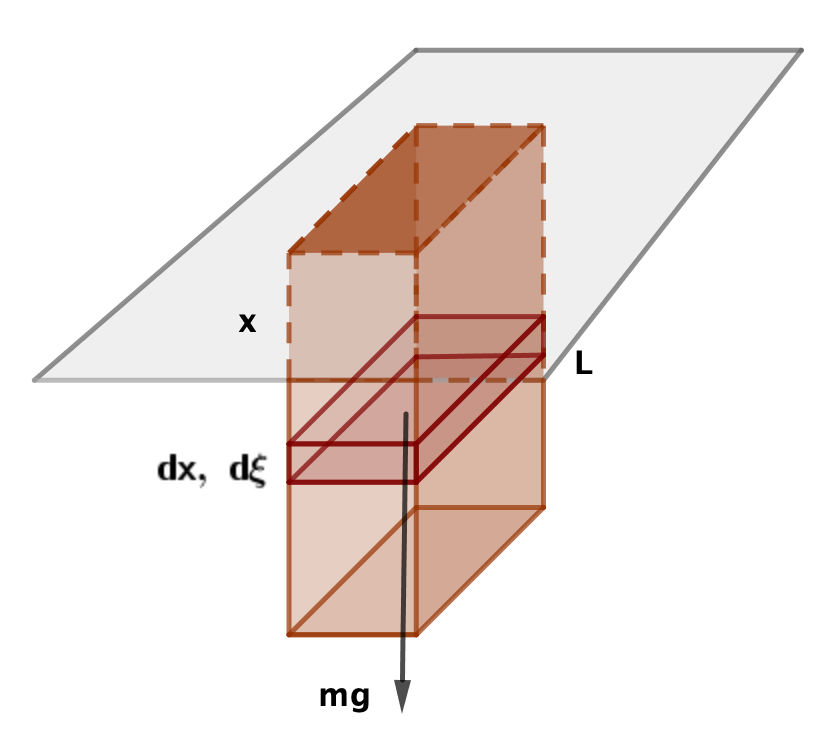
\includegraphics[width=.5\textwidth]{imagenes/imagenes09/T09IM09.png}
\end{figure}	
\end{multicols}


\newpage %*****************************************

\begin{myblock}{?`Qué es la ley de Hooke?}


\vspace{2mm} La Ley de elasticidad de Hooke, o simplemente Ley de Hooke, es el principio físico en torno a la conducta elástica de los sólidos. Fue formulada en 1660 por el científico británico Robert Hooke, contemporáneo del célebre Isaac Newton.

\vspace{2mm} El precepto teórico de esta ley es que el desplazamiento o la deformación sufrida por un objeto sometido a una fuerza, será directamente proporcional a la fuerza deformante o a la carga. Es decir, a mayor fuerza, mayor deformación o desplazamiento, o como lo formuló en latín el propio Hooke: \emph{\textsf{Ut tensio sic vis}}  (``como la extensión, así la fuerza’’).
\vspace{2mm} La Ley de Hooke es sumamente importante en diversos campos, como en la física y el estudio de resortes elásticos (su demostración más frecuente). Es un concepto fundamental para la ingeniería y la arquitectura, la construcción y el diseño, ya que permite prever la manera en que una fuerza prolongada o un peso alterará las dimensiones de los objetos en el tiempo.
\vspace{2mm} Se dice que esta ley fue publicada por Hooke bajo la forma de un misterioso anagrama (ceiiinosssttuv), del cual puede reconstruirse el enunciado en latín de su ley, porque tenía miedo de que alguien pudiera adueñarse ilegalmente de su descubrimiento. Un par de años más tarde, sin embargo, hizo públicos sus hallazgos.


\vspace{2mm} \textcolor{gris}{\small{Robert Hooke (Reino Unido: 1635-1703) físico inglés, considerado uno de los científicos experimentales más importantes de la historia de la ciencia. Sus intereses abarcaron campos tan dispares como la biología, la medicina, la horología (cronometría), la física planetaria, la mecánica de sólidos deformables, la microscopía, la náutica y la arquitectura}\normalsize{.}}	
\end{myblock}







